\chapter{Fundamentação Teórica}
\label{cap:fund}

% figuras estão no subdiretório "figuras/" dentro deste capítulo
\graphicspath{\currfiledir/figuras/}

Nesta parte, há a exposição das definições e histórico de redes sociais, algoritmos de recomendação e as definições matemáticas e computacionais de grafo. Esses três itens relacionam-se intrinsicamente com este trabalho, por isso, buscamos esclarecê-los o suficiente neste capítulo de maneira que as relações destes tópicos com o objetivo geral estejam fundamentadas.


\section{Redes Sociais}

% \begin{itemize}
% \item Histórico de redes sociais
% \item Tipos de redes sociais
% \item Redes parecidas com nosso trabalho
% \item Análises de tempo despendido em redes sociais.
% \end{itemize}

Desde a invenção da internet em 1991, mais e mais aplicações vem sendo criadas para facilitar e estimular os relacionamentos virtuais. As redes sociais virtuais tiveram início em 1997 com o site \emph{Six Degrees}, \citep{terrel17}. \emph{Six Degrees} é nomeado em referência ao estudo de \cite{milgram67}, que teorizava que são necessários seis laços de amizade para que quaisquer pessoas estejam conectadas. \emph{Six Degrees} teve seu fim em 2001, mas iniciou o processo de popularização das redes sociais e é considerado a primeira rede social pois permitia que as pessoas criassem seus perfis individuais e adicionar outros contatos à sua rede. Teve 3,5 milhões de usuários no seu auge.

Entre as precursoras está também a rede especializada em relacionamentos profissionais, \emph{LinkedIn}. Foi criada no final de 2002 e tem, desde então, seu objetivo principal em criar conexões entre profissionais, estudantes e corporações. O \emph{LinkedIn} é, ainda hoje, a rede mais popular neste nicho com mais de 500 milhões de usuários.

A rede mais popular atualmente, segundo \cite{lua19}, é o Facebook com 2,23 milhões de usuários ativos mensalmente. O Facebook foi criado em 2004 como uma rede específica para estudantes da Universidade de Harvard. Em 2006 foi aberta ao público e em 2008 já era a rede social mais visitada do mundo.

Há também redes especializadas em outros tipos de conexão ou outras maneiras de publicar conteúdo. O YouTube é uma rede social especializada na divulgação de vídeos criados pelos usuários. O Twitter, distingue-se das outras redes por iniciar suas atividades permitindo apenas a publicação de textos com, no máximo, 140 caracteres. Este limite foi dobrado posteriormente, mas o foco ainda mantém-se em pequenas postagens.

Por fim, há as redes especializadas em relacionamentos românticos. O Tinder, o Happn e o OKCupid são exemplos de redes sociais direcionadas à criação de relacionamentos íntimos entre os usuários. O sistema desenvolvido neste trabalho enquadra-se nesta categoria pois tem o objetivo de colocar usuários em contato com pessoas desconhecidas que têm potencial para formarem amizades ou até mesmo casais.

No Brasil, 66\% da população tem acesso à internet segundo \cite{wearesocial18}. Dentre os usuários da internet 93\% são ativos em alguma rede social.
Segundo \cite{wearesocial18}, o brasileiro despende, em média, 3h39min por dia em alguma rede social. Este tempo é passado em contato com informações e pessoas de várias culturas diferentes. Muitas vezes as interações despertam sentimentos indesejados e a informação divulgada não é completamente conexa à realidade.

Por essa razão, mais e mais redes sociais oferecem a oportunidade, muitas vezes compulsoriamente, do usuário ser exposto somente à pessoas e conteúdos que tenham afinidade com seu perfil. Na busca por uma experiência agradável, as sugestões de conteúdo e contatos vão ao encontro da necessidade do ser humano de se socializar. E participar de uma rede social, seja ela física ou virtual, faz parte das necessidades básicas apontadas por \cite{Maslow1943}, ao definir uma hierarquia para as necessidades básicas do ser humano.

De uma maneira ou de outra, todas as redes sociais tem seu foco no conteúdo gerado pelos usuários. Porém, grande parte da monetização empregada refere-se à divulgação de peças publicitárias pagas por empresas particulares e públicas. Dentro deste escopo, são utilizados algoritmos que tomam em conta os interesses dos usuários para fazer sugestões de conteúdo publicitário. Há vários métodos para relacionar os dados produzidos pelos usuários para gerar sugestões, sejam elas de conteúdo, publicidade ou novos contatos.

%=====================================================

\section{Algoritmos de Recomendação}

% \begin{itemize}
% \item Como sugerir novos contatos.
% \item Como as outras redes fazem isso.
% 
% \end{itemize}


Quando um usuário acessa um sistema qualquer que lhe oferece itens, por exemplo, livros, um sistema de recomendação pode lhe proporcionar a conveniência de sugerir-lhe um livro mais adequado para o seu gosto quando a quantidade de opções disponíveis é opressivamente vasta, diz \cite{Ricci2010}.

Esses itens, são quaisquer coisas que podem ser sugeridas ao usuário, sejam produtos, serviços, notícias, publicidade, ou, no caso deste trabalho, outros usuários com potencial para tornarem-se amizades.

Para \cite{Ricci2010}, a forma mais simples de um sistema de recomendação é uma lista com itens ordenados pela similaridade com o usuário que receberá a recomendação. Os sistemas de sugestão analisam vários tipos de dados por diversos métodos diferentes para encontrar os itens mais adequados para cada usuário. De acordo com \cite{Ricci2010}, os primeiros algoritmos de recomendação utilizavam dados gerados por recomendações feitas pela comunidade de usuários. Esse método comparava gostos similares entre os usuários e recomendava itens ainda não consumidos por alguns usuários. A este método dá-se o nome de Filtragem Colaborativa \citep{goldberg92}.

Desde os anos 1990, a perseguição por sistemas de recomendações cada vez mais eficientes impulsionou o surgimento do Prêmio Netflix em 2006, \citep{netflix}. Neste concurso, a empresa Netflix propôs pagar um prêmio de US\$1.000.000 para quem elaborasse um sistema que pudesse melhorar em, pelo menos, 10\% a acurácia do sistema que estava em uso à época. O time \emph{BellKor's Pragmatic Chaos}, venceu a disputa empregando diversos algoritmos e métodos de classificação mesclados em um mesmo sistema, \citep{Bell}. 

Entre as possibilidades de métodos e algoritmos que podem ser empregados em um sistema de recomendação, podemos ressaltar, baseados no texto de \cite{Recommendation}, as seguintes:

\begin{itemize}
\item Filtragem colaborativa
\item Filtragem baseada em conteúdo
\item Recomendação baseada em conhecimento
\end{itemize}

A filtragem colaborativa, como já mencionado, leva em conta as preferências já informadas pelos usuários para compará-las e sugerir novas possibilidades de itens. Tem a tendência de sugerir itens que já são apreciados por usuários que, de alguma maneira, já se relacionam, seja por interesses definidos, grupos específicos ou até mesmo por parentesco.

A filtragem baseada em conteúdo toma por verdadeira a afirmação de que os usuários que já demonstraram interesse por um tópico somente serão agradados por tópicos semelhantes e não podem ser instigados por assuntos fora do escopo do que já foi definido como interesse inicialmente. Dessa maneira, o sistema considera de que um usuário que declarou interesse por filmes deve receber sugestões de itens relacionados a este tema. É claro que este método tem a fraqueza de não sugerir novos assuntos que, potencialmente, despertariam o interesse do usuário.

Finalmente, a recomendação baseada em conhecimento,  que toma em conta regras de restrições de interesse definidas no sistema e os aplica à lista de itens disponíveis. Desse modo, os itens são sugeridos a partir do resultado da filtragem realizada a partir das regras definidas. A definição de tais regras passa por análises semânticas do conteúdo disponível no sistema que diga respeito ao usuário. O sistema desenvolvido neste trabalho assemelha-se a uma recomendação baseada em conhecimento no sentido de que a regra definida para relacionar os itens será uma equação determinística que calcula um valor de proximidade entre dois itens.

Os vários métodos de recomendação tem sua acurácia diretamente influenciada pela quantidade de informação disponível sobre os usuários ou gerada pelos usuários. Quanto maior a quantidade de informação disponível, maior a acurácia e, em linhas gerais, menor a performance do sistema, uma vez que o tempo de processamento da informação é incrementado. Por essa razão, boas soluções são baseadas em aprendizado de máquina e inteligência artificial. O emprego dessas tecnologias tem o objetivo de melhorar a performance e a acurácia das sugestões.

%=====================================================

\section{Grafo}
% \begin{itemize}
% \item O que é grafo - \emph{Fonte básica de definição de grafo LIVRO??}
% \item Quantos tipos de grafo existem.
% \item Aplicações comuns de grafo
% \item Algoritmos que usam grafos
% \end{itemize}

O conceito matemático de grafo parte de abstrações de situações da vida real onde objetos ou pessoas representadas por pontos e suas conexões e interações são representadas por linhas \cite{Bondy08}. Numa rede social, as pessoas são esses pontos, que convencionalmente são chamados de nós, e suas relações com outras pessoas são representadas por linhas, chamadas de arestas. Um grafo é uma tripla ordenada $G=(N(G), A(G), \psi _{G})$, que consiste de um conjunto não vazio $N(G)$ de nós, um conjunto $A(G)$, diferente de $N(G)$, de arestas, e uma \emph{função de incidência} $\psi_{G}$ que associa a cada nó de $G$ um par não ordenado de nós de $G$. Se $e$ é uma aresta de $G$ e $u$ e $v$ são arestas de tal modo que $\psi_{G}(e) = un$, então $e$ é dito que \emph{une} $u$ e $n$ \cite{Bondy08}.

\emph{Exemplo}

\begin{equation}
G=(N(G), A(G), \psi _{G})
\label{eq:grafo}
\end{equation}

\emph{onde}

\begin{equation}
N(G)={n_{1}, n_{2}, n_{3}, n_{4}, n_{5}}
\label{eq:grafo2}
\end{equation}

\emph{e $\psi_{G}$ é definido por}

\begin{equation}
\begin{split}
\psi_{G}(a_{1}) = n_{1}n_{2}, \psi_{G}(a_{2} = n_{2}n_{3}, \psi_{G}(a_{3}) = n_{3}n_{3}, \psi_{G}(a_{4}) = n_{2}n_{4} \\
\psi_{G}(a_{5}) = n_{2}n_{4}, \psi_{G}(a_{6} = n_{4}n_{5}, \psi_{G}(n_{8}) = n_{2}n_{5}, \psi_{G}(a_{4}) = n_{2}n_{4}
\label{eq:grafo3}
\end{split}
\end{equation}

Grafos têm este nome pois podem ser representadas graficamente, segundo \cite{Bondy08}. A Figura \ref{fig:grafo}, é um diagrama que representa um grafo com 5 nós e 6 arestas. Nesta Figura, os nós têm identificação - letras - e as arestas tem um \emph{peso}. O peso das arestas pode ser usado para representar a força da ligação entre os nós ou até mesmo a distância entre os nós. A convenção tomada neste caso depende do contexto e da aplicação do grafo.

\begin{figure}[!htb]
\centering
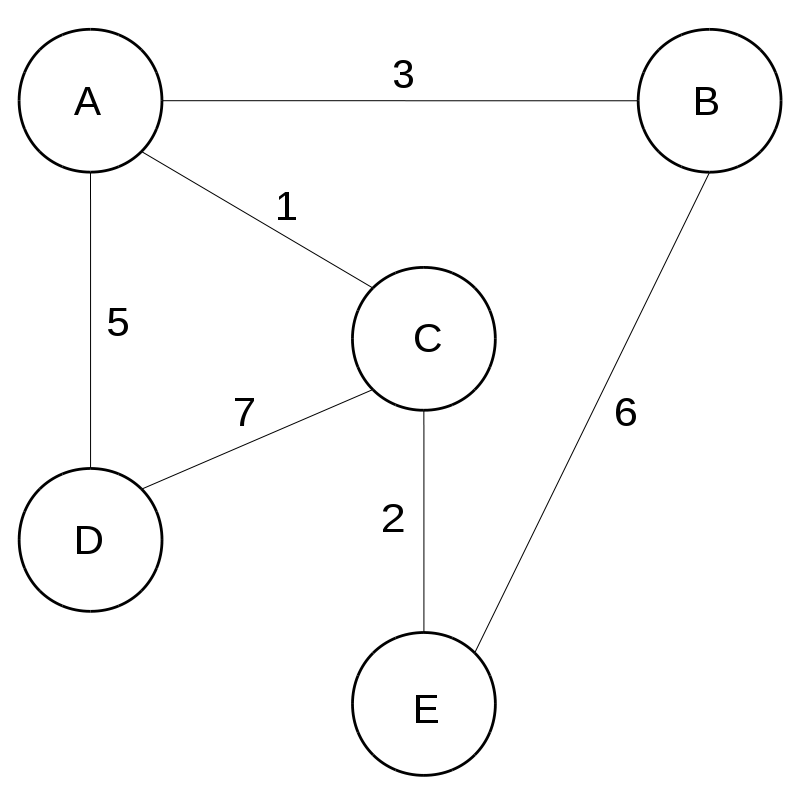
\includegraphics[width=12cm]{grafo.png}
\caption{Um grafo com 5 nós e 6 arestas.}
\label{fig:grafo}
\end{figure}

Quando a relação entre dois nós é simétrica, ou seja, a relação entre o nó $A$ e o nó $B$ é idêntica, diz-se que o grafo é \emph{não orientado}. Quando a relação entre dois nós é assimétrica, portanto, $A$ tem uma relação com $B$, mas essa relação não equivale a $B$ para $A$, tem-se um \emph{dígrafo} ou um \emph{grafo orientado}.

Este trabalho utiliza o grafo não orientado pois este bem representa as relações de amizade recíprocas. Tal decisão é tomada pois, quando da sugestão de um novo contato, ambos vão ser apresentados reciprocamente, estabelecendo, portanto, uma relação mútua de interação.

Diversas áreas da ciência, desde a biologia à linguística, utilizam grafos para representar dados. A representação de objetos e suas relações é uma ferramenta frequente em várias pesquisas.

Na ciência da computação, o grafo é a uma estrutura de dados amplamente frequente e existem centenas de problemas computacionais definidos com o seu uso \cite{Cormen2009}. Um caso tradicional com solução utilizando grafos é a do caixeiro viajante. Neste problema, os nós do grafo são as localidades e as arestas têm o peso equivalente à distância entre as cidades. \citep{Dijkstra1959}, propôs o primeiro algoritmo para encontrar o caminho mais curto entre dois nós de um grafo. O algoritmo encontra um caminho curto, mas não necessariamente o mais curto. Vários trabalhos são realizados ainda hoje na busca pelo caminho mais curto em um grafo. Muitos desses trabalhos são baseados no algoritmo de Dijkstra.

Como estrutura de dados computacionais, existem várias modelagens conhecidas para representação de um grafo. \citep{Cormen2009}, cita duas formas fundamentais:

\begin{itemize}
\item A lista de adjacência
\item A matriz de adjacência
\end{itemize}

\begin{figure}[!htb]
\centering
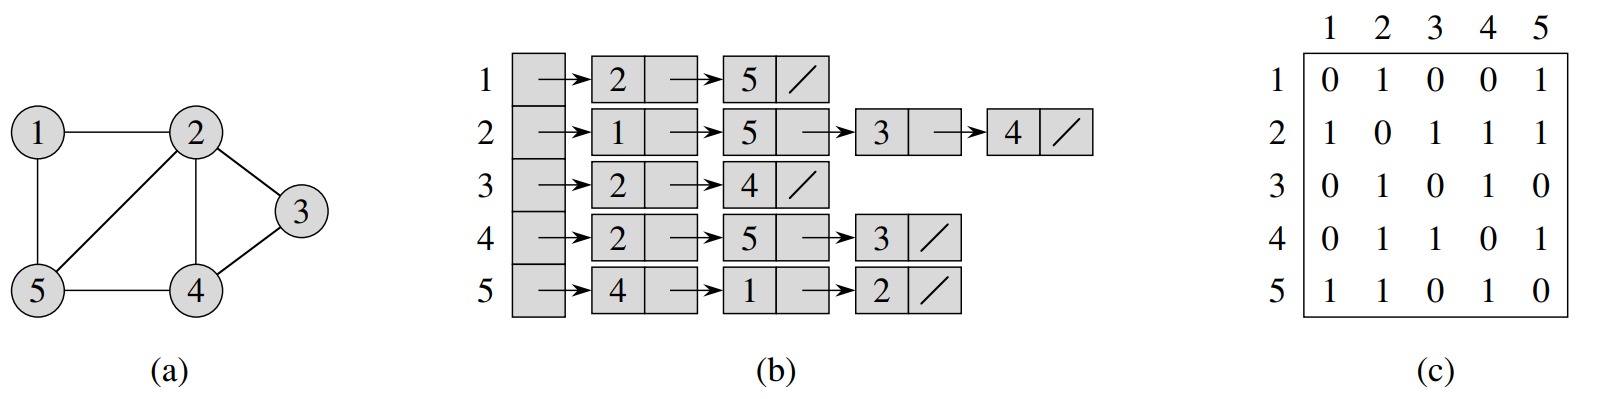
\includegraphics[width=16cm]{represent_grafo.png}
\caption{Duas representações de um grafo não direcionado. (\textbf{a}) Um grafo G com cinco nós e sete arestas. (\textbf{b}) A representação de uma lista de adjacência de G. (\textbf{c}) A representação de uma matriz de adjacência. Fonte: \cite{Cormen2009}, tradução dos autores.}
\label{fig:represent_grafo}
\end{figure}


\begin{figure}[!htb]
\centering
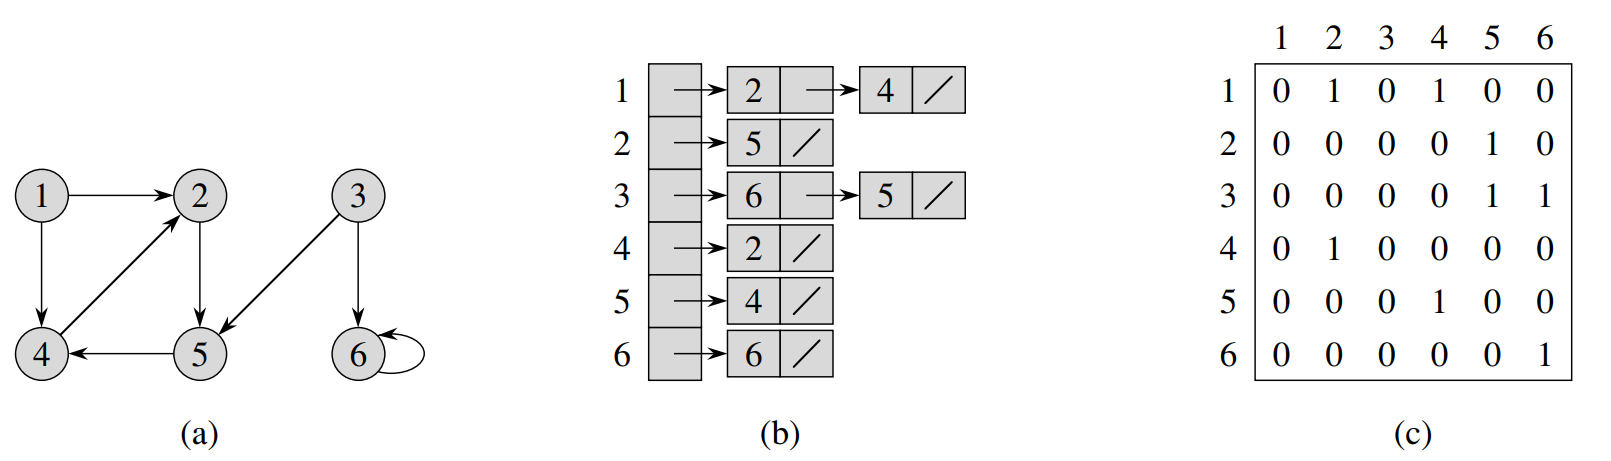
\includegraphics[width=16cm]{represent_grafo_ND.png}
\caption{Duas representações de um grafo direcionado. (\textbf{a}) Um grafo G com seis nós e oito arestas. (\textbf{b}) A representação de uma lista de adjacência de G. (\textbf{c}) A representação de uma matriz de adjacência. Fonte: \cite{Cormen2009}, tradução dos autores.}
\label{fig:represent_grafo_ND}
\end{figure}

\FloatBarrier

A Figura \ref{fig:represent_grafo}, ilustra um grafo $G$ como um diagrama, como uma lista de adjacência e como uma matriz de adjacência. A implementação computacional de um grafo pode ser a partir de uma lista de adjacência. Desse modo Um grafo $G = (N, E)$ consiste de uma lista de listas de nós, uma lista para cada nó em N. Para cada nó em G, tem-se uma lista dos nós vizinhos. Essa lista também pode conter somente um ponteiro para os nós vizinhos. Normalmente é suficiente armazenar os nós vizinhos em ordem arbitrária pois será o peso da aresta que determinará uma hierarquia entre os nós vizinhos, não a ordem pela qual eles foram adicionados nem qualquer outro atributo.
